\documentclass[11pt,a4paper,]{article}
\usepackage{float}
  \usepackage[]{mathpazo}
  \usepackage{setspace}

%\usepackage[T1]{fontenc} %RK added
\usepackage{lmodern} %RK added

\usepackage{amssymb,amsmath}
\usepackage{ifxetex,ifluatex}
\usepackage{fixltx2e} % provides \textsubscript
\ifnum 0\ifxetex 1\fi\ifluatex 1\fi=0 % if pdftex
\usepackage[T1]{fontenc}
\usepackage[utf8]{inputenc}
\usepackage{csquotes}
  \else % if luatex or xelatex
  \usepackage{unicode-math}
  \defaultfontfeatures{Ligatures=TeX,Scale=MatchLowercase}
              \fi
% use upquote if available, for straight quotes in verbatim environments
\IfFileExists{upquote.sty}{\usepackage{upquote}}{}
% use microtype if available
\IfFileExists{microtype.sty}{%
  \usepackage[]{microtype}
  \UseMicrotypeSet[protrusion]{basicmath} % disable protrusion for tt fonts
}{}
\PassOptionsToPackage{hyphens}{url} % url is loaded by hyperref
\usepackage{fancybox}
  \usepackage[unicode=true]{hyperref}
  \hypersetup{
    pdfauthor={Ryan N. Kinzer (Research Division, Department of Fisheries Resources Management)},
          pdftitle={Snake River Steelhead Kelt Summary},
            %                pdfborder={0 0 0},
          breaklinks=true}
                
\urlstyle{same}  % don't use monospace font for urls
\usepackage[margin=1in]{geometry}

\usepackage[style=authoryear-comp,backend=biber, natbib=true,]{biblatex}
\addbibresource{kelt\_summary.bib}
\addbibresource{kelt\_summary\_package.bib}

\usepackage{longtable,booktabs}
% Fix footnotes in tables (requires footnote package)
\IfFileExists{footnote.sty}{\usepackage{footnote}\makesavenoteenv{long table}}{}
\usepackage{graphicx,grffile}
\makeatletter
\def\maxwidth{\ifdim\Gin@nat@width>\linewidth\linewidth\else\Gin@nat@width\fi}
\def\maxheight{\ifdim\Gin@nat@height>\textheight\textheight\else\Gin@nat@height\fi}
\makeatother
% Scale images if necessary, so that they will not overflow the page
% margins by default, and it is still possible to overwrite the defaults
% using explicit options in \includegraphics[width, height, ...]{}
\setkeys{Gin}{width=\maxwidth,height=\maxheight,keepaspectratio}
\IfFileExists{parskip.sty}{%
\usepackage{parskip}
}{% else
\setlength{\parindent}{0pt}
\setlength{\parskip}{6pt plus 2pt minus 1pt}
}
\setlength{\emergencystretch}{3em}  % prevent overfull lines
\providecommand{\tightlist}{%
  \setlength{\itemsep}{0pt}\setlength{\parskip}{0pt}}
\setcounter{secnumdepth}{5}

% set default figure placement to htbp
\makeatletter
\def\fps@figure{htbp}
\makeatother

\title{Snake River Steelhead Kelt Summary \vspace{0.5cm}}

\author{\Large \bf{Ryan N. Kinzer}\vspace{0.05in} \newline\normalsize\emph{Research Division, Department of Fisheries Resources Management}  }

%% MONASH STUFF

%% CAPTIONS
\RequirePackage{caption}
\DeclareCaptionStyle{italic}[justification=centering]
 {labelfont={bf},textfont={it},labelsep=colon}
\captionsetup[figure]{style=italic,format=hang,singlelinecheck=true}
\captionsetup[table]{style=italic,format=hang,singlelinecheck=true}

%% FONT
\usepackage{bm,url}

%% HEADERS AND FOOTERS
\RequirePackage{fancyhdr}
\pagestyle{fancy}
\lfoot{}\cfoot{}\rfoot{}
\lhead{\textsf{Kelt Summary}} % was title
\rhead{\textsf{\thepage}}
\setlength{\headheight}{15pt}
\renewcommand{\headrulewidth}{0.4pt}
\fancypagestyle{plain}{%
\fancyhf{} % clear all header and footer fields
\fancyfoot[C]{\sffamily\thepage} % except the center
\renewcommand{\headrulewidth}{0pt}
\renewcommand{\footrulewidth}{0pt}}

%% MATHS
\RequirePackage{bm,amsmath}
\allowdisplaybreaks

%% GRAPHICS
\RequirePackage{graphicx}
\setcounter{topnumber}{2}
\setcounter{bottomnumber}{2}
\setcounter{totalnumber}{4}
\renewcommand{\topfraction}{0.85}
\renewcommand{\bottomfraction}{0.85}
\renewcommand{\textfraction}{0.15}
\renewcommand{\floatpagefraction}{0.8}

%\RequirePackage[section]{placeins}

%% SECTION TITLES
\RequirePackage[compact,sf,bf]{titlesec}
\titleformat{\section}[block]
  {\fontsize{15}{17}\bfseries\sffamily}
  {\thesection}
  {0.4em}{}
\titleformat{\subsection}[block]
  {\fontsize{12}{14}\bfseries\sffamily}
  {\thesubsection}
  {0.4em}{}
\titlespacing{\section}{0pt}{*3}{*1}
\titlespacing{\subsection}{0pt}{*1}{*0.5}

%% LINE AND PAGE BREAKING
\sloppy
\raggedbottom
\usepackage[bottom]{footmisc}
\clubpenalty = 10000
\widowpenalty = 10000
\brokenpenalty = 10000
\RequirePackage{microtype}

%% HYPERLINKS
\RequirePackage{xcolor} % Needed for links
\definecolor{darkblue}{rgb}{0,0,.6}
\RequirePackage{url}

\makeatletter
\@ifpackageloaded{hyperref}{}{\RequirePackage{hyperref}}
\makeatother
\hypersetup{
     citecolor=0 0 0,
     breaklinks=true,
     bookmarksopen=true,
     bookmarksnumbered=true,
     linkcolor=darkblue,
     urlcolor=blue,
     citecolor=darkblue,
     colorlinks=true}

\usepackage[showonlyrefs]{mathtools}

%% BIBLIOGRAPHY

\makeatletter
\@ifpackageloaded{biblatex}{}{\usepackage[style=authoryear-comp, backend=biber, natbib=true]{biblatex}}
\makeatother
\ExecuteBibliographyOptions{bibencoding=utf8,minnames=1,maxnames=3, maxbibnames=99,dashed=false,terseinits=true,giveninits=true,uniquename=false,uniquelist=false,doi=false, isbn=false,url=true,sortcites=false}
\DeclareFieldFormat{url}{\texttt{\url{#1}}}
\DeclareFieldFormat[article]{pages}{#1}
\DeclareFieldFormat[inproceedings]{pages}{\lowercase{pp.}#1}
\DeclareFieldFormat[incollection]{pages}{\lowercase{pp.}#1}
\DeclareFieldFormat[article]{volume}{\mkbibbold{#1}}
\DeclareFieldFormat[article]{number}{\mkbibparens{#1}}
\DeclareFieldFormat[article]{title}{\MakeCapital{#1}}
\DeclareFieldFormat[article]{url}{}
%\DeclareFieldFormat[book]{url}{}
%\DeclareFieldFormat[inbook]{url}{}
%\DeclareFieldFormat[incollection]{url}{}
%\DeclareFieldFormat[inproceedings]{url}{}
\DeclareFieldFormat[inproceedings]{title}{#1}
\DeclareFieldFormat{shorthandwidth}{#1}
%\DeclareFieldFormat{extrayear}{}
% No dot before number of articles
\usepackage{xpatch}
\xpatchbibmacro{volume+number+eid}{\setunit*{\adddot}}{}{}{}
% Remove In: for an article.
\renewbibmacro{in:}{%
  \ifentrytype{article}{}{%
  \printtext{\bibstring{in}\intitlepunct}}}
\AtEveryBibitem{\clearfield{month}}
\AtEveryCitekey{\clearfield{month}}
\makeatletter
\DeclareDelimFormat[cbx@textcite]{nameyeardelim}{\addspace}
\makeatother
\renewcommand*{\finalnamedelim}{%
  %\ifnumgreater{\value{liststop}}{2}{\finalandcomma}{}% there really should be no funny Oxford comma business here
  \addspace\&\space}


%%% Change title format
\usepackage{color,titling,framed}
\usepackage[absolute,overlay]{textpos}
\setlength{\TPHorizModule}{1cm}
\setlength{\TPVertModule}{1cm}

\pretitle{%
%
\begin{textblock}{4}(2,0.8)
\includegraphics[height=2.0cm]{NPT.png}\end{textblock}%
\begin{textblock}{4}(17,0.8)
\includegraphics[height=2.0cm]{DFRM.png}\end{textblock}%
%\begin{textblock}{4}(16.5,0.8)
\includegraphics[trim=53 0 0 0, clip=true,height=1.5cm]{NPT.png}\end{textblock}%
\vspace*{-1.0cm}%-0.6

\LARGE\bfseries}
\posttitle{\vspace*{0.3cm}\par}
\preauthor{\large}
\postauthor{\hfill\par}
\predate{\hfill\small}
\postdate{}

\raggedbottom

\usepackage[australian]{babel}
\date{10 January, 2022}

\usepackage{booktabs}
\usepackage{longtable}
\usepackage{array}
\usepackage{multirow}
\usepackage{wrapfig}
\usepackage{float}
\usepackage{colortbl}
\usepackage{pdflscape}
\usepackage{tabu}
\usepackage{threeparttable}
\usepackage{threeparttablex}
\usepackage[normalem]{ulem}
\usepackage{makecell}
\usepackage{xcolor}
\usepackage{fontspec}
\usepackage{multicol}
\usepackage{hhline}
\usepackage{hyperref}


\begin{document}


  \vspace*{0cm}
  \definecolor{shadecolor}{RGB}{255,255,255} %210
  \begin{snugshade}%\sffamily
  \maketitle
  \end{snugshade}\vspace*{0.5cm}
  \definecolor{shadecolor}{RGB}{248,248,248} %248

\hbox{\vrule height .2pt width 16cm}

%\hbox{\vrule height .2pt width 16cm} % RK added

\setstretch{1.2}


\hypertarget{background}{%
\section{Background}\label{background}}

Unlike the semelparous life-history of salmon \emph{Oncorhynchus spp.}, anadromous steelhead trout \emph{O. mykiss} in the Pacific Northwest are capable of iteroparity, and potentially contribute to multiple brood years before death \autocite{quinnBehaviorEcologyPacific2018}. To complete multiple spawning events, post-spawned steelhead, often in poor physical condition, immediately emigrate downstream towards the ocean and the abundant food sources to recover physiologically \autocite{penneyProximateCompositionEnergy2014}. These post-spawned and downstream emigrating steelhead are commonly referred to as kelt \autocite{quinnBehaviorEcologyPacific2018}. If successful in reaching the ocean, kelt recover for one or two years before migrating upstream again to become a repeat spawner \autocite{need_citation}. Repeat spawning (i.e., iteroparity) is known to buffer against negative environmental stochasticity, increase genetic diveristy and may provide large boosts to population productivity. As such, and given the current downward abundance trends of Pacific Northwest steelhead \autocite{need_citation}, understanding the limiting factors to steelhead kelt and repeat spawner survival is essential to preserving steelhead populations and meeting recovery goals.

In the Columbia River and Snake River basins, steelhead kelt and repeat spawners are primarily tracked using information collected at hydrosystem facilities. Typically, researchers identify kelt and repeat spawners with radio telemetry studies \autocite{wertheimerDownstreamPassageSteelhead2005}, biological samples (e.g., scales, genetics) collected from a portion of fish trapped at Bonneville Dam (BON) or Lower Granite Dam (LGD) facilities \autocite{copelandPatternsIteroparityWild2019,matalaWhatGoesDoes2016,lawryWildAdultSteelhead2020,hessDifferentialAdultMigrationtiming2016}, or with passive integrated transponder (PIT) tag detections as fish pass the hydrosystems \autocite{copelandPatternsIteroparityWild2019,keeferIteroparityColumbiaRiver2008}. Using these tools, researchers are able to track migration routes, timing, survival, and estimate the abundance of kelt and repeat spawners within the total steelhead return. \textcite{wertheimerDownstreamPassageSteelhead2005} used radio-tags to find kelt survival from Lower Granite Dam (LGD) to below Bonneville Dam (BON) was only 4.1\% in 2001 and 15.6\% in 2002. And \textcite{matalaWhatGoesDoes2016} used mixed stock analysis to proportion kelt and repeat spawners captured at LGD into genetic stock groups, finding greater than 80\% of kelt assigned to A-run type genetic stocks as compared to 70\% of the returning repeat spawners, while the remainder of the captured steelhead kelt and repeat spawners assigned to B-run stocks. More recently, \textcite{copelandPatternsIteroparityWild2019} used a combination of genetic analysis and detections of passive integrated transponder (PIT) tags at LGD and BON to determine survival of kelt emigrating downstream and repeat spawners returning upstream. \textcite{copelandPatternsIteroparityWild2019} determined between 2010 and 2015 kelt survival from initial spawning to BON ranged from 10\%-44\%, 2\%-14\% for repeat spawners returning from the ocean to BON, and then found a fairly high conversion rate (\textgreater65\%) of repeat spawners moving from BON to LGD.

Although most critical information regarding steelhead kelt and repeat spawner survival and abundance is largely known as adults emigrate past LGD towards the ocean, understanding the proportion of fish attempting to kelt, their post-spawning survival or their limiting factors is more elusive. The estimation of kelt metrics upstream of LGD requires the observation of fish immediately after spawning, and prior to any potential downstream migration mortality. Until recently, observations of kelt were limited to only those surviving to reach mainstem observation points (e.g., Lower Granite Dam). However, in the last 10-years in-stream PIT-tag detection systems (IPTDS) have become a wide-spread tool to conduct salmon and steelhead research in the Snake River Basin \autocite{kinzerSnakeRiverBasin2020,dobosUnderstandingLifeHistory2020,briana.knothIDAHOADULTSTEELHEAD2018}.

Beginning with spawn year 2010, fish managers have relied on the network of IPTDS across the Snake River Basin to gain abundance estimates of steelhead reaching tributary spawning locations \autocite{seePITTagBased2016,kinzerREPORTNOAAFISHERIES2020}. The method begins by estimating the total number of unique adult steelhead passing LGD as they migrate toward spawning areas \autocite{seeStateSpaceModelEstimate2021}, and a systematic sample of PIT-tagged fish passing LGD. The total number of fish passing LGD is then partitioned into spawning areas using a branch-occupancy model described by \textcite{seePITTagBased2016} and \textcite{waterhouseBayesianNestedPatch2020}, and the PIT-tag interrogation data collected at IPTDS. Using the same systematic sample of PIT-tagged fish, and estimated spawner abundances, we hypothesize that downstream emigrating kelt survival and abundance can be estimated at the spawning location. Thus, expanding our knowledge of steelhead kelt distribution, abundance, and survival using existing infrastructure, available data, and building from the previous work of \textcite{seePITTagBased2016} and \textcite{seeStateSpaceModelEstimate2021}. Our work fills an information gap regarding this potentially critical and previously unknown adult steelhead life-history stage (i.e., spawning grounds to LGD), and combined with the findings of \textcite{copelandPatternsIteroparityWild2019} can be used to better manage and recover steelhead populations.

Generally, we seek to better understand the complex kelting life-history of anadromous Snake River steelhead. Our main objective is to provide guidance to fish managers as they review steelhead limiting factors, consider recovery actions, and prioritize life-history stages or populations needing the most assistance. Specifically, we aim to answer three kelt related research questions: (1) what proportion of adult steelhead escaping and spawning in Snake River Basin populations attempt the kelt life-history (i.e., emigrate from spawning area), (2) determine if correlations between kelting rates and demographic characteristics (i.e., age, sex, stock, etc.) exist, and if the rates differ across populations, and (3) what is the survival of kelt from the spawning grounds to LGD and BON? The methods and results presented here provide an analytical framework intended to answer the above stated research questions. The methods section first describes PIT-tag interrogation data as a potential data source, and discusses how interrogation data is processed to classify different adult steelhead life-history stages and summarize PIT-tag observations. Then, a statistical model is described which is capable of expanding PIT-tag observations by detection probabilities to estimate population specific kelting rates and downstream migration survival for spawning populations. Finally, spawn year 2021 data summaries are reported along with tentative model results. Together, the methods and results provide a proof of concept, share currently available information, and begin to illustrate patterns that may emerge after additional modelling using multiple years of data.

\hypertarget{methods}{%
\section{Methods}\label{methods}}

\hypertarget{data-source}{%
\subsection{Data Source}\label{data-source}}

To begin answering our three research questions we evaluated PIT-tag observations from a random sample of natural-origin adult steelhead captured at Lower Granite Dam during spawn year 2021. We generated PIT-tag observations by first developing a list of natural-origin fish with \emph{valid} PIT-tag codes collected at the Lower Granite Dam adult trap beginning July 1st and ending June 30th of the spawn year \autocite{need_citation}. Fish origin was determined by the presence of an adipose fin and the failure to genetically assign the fish to a hatchery stock using parentage based tagging \autocite{IDFGcitation,steeleValidationParentagebasedTagging2013}. PIT-tag codes were then deemed valid if a natural-origin fish was trapped while ascending the LGD fish ladder during a systematic sub-sampling period. Once a valid tag list was developed, all PIT-tag interrogations for each tag code was obtained using the complete tag history query from the \href{https://www.ptagis.org}{PTAGIS} website and processed using computer algorithms.

The full dataset was initially processed with the \texttt{PITcleanr::compression()} function \autocite{R-PITcleanr} developed for the R statistical language software \autocite{R-base}. The \texttt{PITcleanr::compression()} function and the supplied configuration file collapsed multiple rows of PIT-tag interrogations at the same location and during a similar time-period, into a single row of data. The resulting data contained the PIT-tag code, observation location (i.e., node), and the minimum and maximum date/time of observations. Thus, removing any unnecessary and redundant information from the full dataset. The supplied configuration file was constructed using \texttt{PITcleanr::buildConfig} which was then altered to group detection nodes (i.e., a group of PIT-tag antennas or sites) into Lower Columbia, Mid-Columbia, Upper Columbia, and Lower Snake River categories. All detection nodes within the Snake River steelhead distinct population segment (DPS) remained unique, to facilitate the assignment of detections to distinct spawning locations, or populations. We then truncated the compressed observations to include only observations occurring after an upstream migrating steelhead was initially detected at the LGD trap (i.e., we removed all juvenile and adult observations prior to reaching LGD as a returning adult).

Next, we used the \texttt{PITcleanr::addDirection()} function with a supplied parent-child table of nodes to assign detection pathways to each PIT-tag observation, and to define movements as either forward or backward. The parent-child table was pre-constructed and informed the function of each detection pathway (i.e., all possible detection nodes), in the upstream direction, that a fish would pass to reach the actual node of observation. Once the order of detection nodes was known, the \texttt{PITcleanr::addDirection()} function labeled observations as either a forward (i.e., upstream) or backward (i.e., downstream) movement.

Then, using the travel pathways and directional movements, each PIT-tag code, or fish, was assigned to one of three LGD migration patterns: typical, fallback, or reascension; and if the fish was observed as a kelt. The migration patterns at LGD described how an upstream migrating steelhead navigated the dam while traveling to the spawning grounds, and enable us to compare the kelting rates and survival of each group. A typical LGD migration pattern was assigned to PIT-tags observed at the LGD trap and ladder once; thus, assuming the fish ascended the ladder and moved directly towards the spawning grounds. The fallback migration pattern was assumed if a single LGD trap or ladder detection was observed, and then was immediately followed by a PIT-tag detection at GRS, GRJ, or any PIT-tag observation site downstream of LGD (e.g., Bonneville Dam corner collector, Preist Rapids ladder, Tucannon River). A reascension fish was assumed to have multiple LGD ladder ascension, and were identified by either PIT-tag interrogations in the ladder or upstream of LGD following a detection GRS, GRJ or another downstream location. We assumed a fish was a kelt on the spawning grounds if there was a backward moving interrogation at an IPTDS at least \textbf{X} days after the latest forward movement within the same detection pathway. Kelt observations at LGD was determined if a PIT-tag observation occurred at GRS, GRJ during the months of April, May and June, and the observation was at least 5 days after the last upstream detection on the spawning grounds (\textbf{maybe this should be changed to X number of days after the last GRA detection to distinguish from fallback, b/c some kelt can travel from spawning grounds to GRA in less time than 5 days}). We determined a kelt observation at BON if an interrogation at BON existed at any date later then the initial detection of upstream migrating fish at LGD.

Finally, we processed the dataset with \texttt{PITcleanr::filterDetections} which iteratively cycled through each PIT-tag code and observations to determine the final spawn location and valid upstream moving detections. This step was necessary for future modeling with the branch occupancy model \autocite{seePITTagBased2016}, and helped ensure that PIT-tagged fish were placed into the correct spawning area, when interrogations and detection pathways indicated a fish was observed in multiple areas. The function first identified if more than one detection pathway existed within the series of observations. If more than one pathway existed, the series of PIT-tag interrogations were flagged for a biologist to determine the correct spawning location based on known spawn timing and behavior for each population. If only one pathway was detected in the complete series of observations, the spawning location or population was assigned based on the furthest upstream detection node.

\hypertarget{data-processing-steps}{%
\subsubsection{Data Processing Steps}\label{data-processing-steps}}

\begin{enumerate}
\def\labelenumi{\arabic{enumi}.}
\tightlist
\item
  Prepare parent-child table starting with Bonneville Dam as the root observation site, with all other sites upstream.
\item
  Build configuration file which maps PTAGIS sites-antennas to detection nodes.
\item
  Compress PTAGIS files and add travel direction to each observation using PITcleanR and custom parent-child table, then add steelhead life-stage (i.e., spawner, kelt, repeat spawner) to each observation.
\item
  Process spawner observations only using PITcleanR's \texttt{filterDetections} to eliminate observations in multiple pathways. Kelt and repeat spawner observations are often in different pathways, so these need to be removed before running the function, and then later called a valid observation.
\end{enumerate}

\hypertarget{analytical-model}{%
\subsection{Analytical Model}\label{analytical-model}}

To model the kelting rate and survival rate between observation points we summarized the observation dataset into a more simple capture-history matrix and modeled survival using a Cormack-Jolly Seber model \autocite{lebretonModelingSurvivalTesting1992}. The capture-history matrix included a row for each valid PIT-tag and four columns containing a 1, indicating a PIT-tag observation, and a 0 for a non-observation. The four columns pertained to: (1) PIT-tag codes observed moving upstream at the spawning location, (2) kelt observed moving downstream at the spawning location, (3) kelt observed at LGD, and (4) kelt observed at BON. Each PIT-tag code within the matrix also included group and individual covariate information to allow for differing survival and PIT-tag detection rates. Covariates may include spawning population, genetic stock, kelt migration timing (\textbf{not sure this can be done}), sex, age, size, or other metrics that can be assigned to each fish.

We constructed a state-space Cormack-Jolly-Seber model \autocite{royleHierarchicalModelingInference2008} model to estimate population specific (\(p\)) survival rates and account for unobserved PIT-tags due to varying detection efficiencies. Using this approach, we estimate survival from the true unknown state (\(z_{i,t}\)) of individual fish \(i\) passing a location at time \(t\) with the following process model:

\[
z_{i,p,t+1}|z_{i,p,t} \sim Bernoulii(z_{i,p,t} \phi_{p,t}).
\]
In this formulation, \(\phi_{p,t}\) represents the population survival probability for all fish from time \(t - 1\) to time \(t\). The probability of survival for an individual fish is then the product of the state variable \(z_{i,p,t}\) and survival, where \(z_{i,p,t}=1\) if a fish is alive at time \(t\), and \(z_{i,p,t}=0\) if the fish is dead. In absence of a 100\% detection rates of downstream moving kelt, we estimated the state process using the imperfect observation data (\(y_{i,p,t}\)) in the capture history matrix. Given an individual is truely alive at time \(t\), we can estimate the probability of detection with the observation model:

\[
y_{i,p,t}|z_{i,p,t} \sim Bernoulii(z_{i,p,t} \rho_{p,t}).
\]
Within the observation model, the detection probability of a fish within population \(p\) given they are alive at time \(t\) is represented by \(\rho_{p,t}\).

\emph{Specific modelling details need included; such as, how population differences are modeled (i.e., fixed vs.~random effects), and how individual covariate effects are included.}

\hypertarget{results}{%
\section{Results}\label{results}}

\hypertarget{todo}{%
\subsection{TODO}\label{todo}}

\begin{itemize}
\tightlist
\item
  need to test if kelt rates and survival is equal across all populations\ldots.Chi squared test for expected/observed counts
\item
  need summary of downstream detection locations and timeframe to solidify our kelt calls, for instance, show not many tags observed in upper-c or mid-c during plausible spawning times, and that most detections are during kelt/repeat spawning times
\item
  need amount of time from spawning obs. to kelt obs in pop, and then at hydro-system
\item
  run-timing of migrant spawners at LGR and pop.
\item
  estimate proportion of spawners surviving to LWG from each population, by pooling all detections.
\end{itemize}

\hypertarget{data-summary}{%
\subsection{Data Summary}\label{data-summary}}

\hypertarget{how-many-lgd-tags-were-observed-on-spawning-grounds}{%
\subsubsection{How many LGD tags were observed on spawning grounds?}\label{how-many-lgd-tags-were-observed-on-spawning-grounds}}

In spawn year 2021, the Lower Granite adult trap released 4,033 valid tags for later detection at IPTDS, hatcheries and other downstream hydrosystem facilities. Of the valid tags released from LGD, approximately 57\% (n = 2,315) were determined to spawn upstream of LGD, 3\% (n = 113) were presumed to spawn downstream of LGD, and 40\% (1,605) had an unknown spawn location (Table \ref{tab:sum-kelt-loc}). The majority of the fish released from LGD assigned to the Grande Ronde (GRROND) genetic stocks group (Figure \ref{fig:sum-gsi}. The Upper Salmon (UPSALM), Lower Snake (LSNAKE), and Upper Clearwater (UPCLWR) GSI groups were the next numerous for fish released and within the valid list. PIT-tag observation locations suggested spawning occurred in most of the Snake River steelhead populations (Table \ref{tab:sum-kelt-pop}). Most tags detected on the spawning grounds were observed within the South Fork Clearwater River population (n = 511). The second highest number of tags (n = 246) were seen in the Salmon River upper mainstem population (includes detections from USI and USE PIT-tag arrays). The fewest PIT-tag detections were seen within the Secesh River population (n = 6). Of the PIT-tagged fish detected within population spawning areas, many of them were assigned to non-concordant genetic stocks (Figure \ref{fig:sum-gsi-pop}). Suggesting spawning fish are straying between populations to a high degree, and/or genetic assignment is not reflective of actual spawner abundance in a population area. Thus, making previous conclusions regarding population life-history or kelting/survival rate differences hard to interpret and generalize to actual spawning populations if methods were based primarily on genetic stock assignments.

\hypertarget{what-proportion-of-tags-observed-on-the-spawning-grounds-were-later-detected-as-kelt-at-lower-granite-dam-or-downstream}{%
\subsubsection{What proportion of tags observed on the spawning grounds were later detected as kelt at Lower Granite Dam or downstream?}\label{what-proportion-of-tags-observed-on-the-spawning-grounds-were-later-detected-as-kelt-at-lower-granite-dam-or-downstream}}

At this time, we are still unable to answer how many kelt are observed leaving the spawning grounds. Methods are currently being developed to more efficiently identify these downstream migrating kelt.

The number of PIT-tags observed on the spawning grounds and later detected as steelhead kelt was 410 unique tags (Table \ref{tab:sum-kelt-loc}). Of these observed kelt tags, 306 tags were observed at LGD and 155 were observed at BON.

A minimum rate of kelting plus survival to LGD, for known upstream spawners, was approximately 18\%. Of the 1,605 tags that were never observed on the spawning grounds after passing LGD, 23\% were later seen heading downstream as kelt. We observed the highest minimum kelting plus survival rate for fish spawning in the Secesh River population (n = 6; 83.3\%) and the lowest rate for fish spawning in the South Fork Clearwater River population (n = 511; 4.9\%). After reaching LGD, the minimum survival of kelt to Bonneville Dam ranged from 4\% for the South Fork Clearwater River spawners, to 66.7\% for the Clearwater River lower mainstem and Big, Camas, and Loon Creek populations.

Detection rates of tags on the spawning grounds is different, but they should be similar for all groups at LGD and BON, therefor; survival to BON should be relative to one another.

\begin{figure}
\includegraphics[width=33.33in]{../../SnakeBasinFishStatus/Figures/site_map} \caption{Snake River steelhead PIT-tag detection sites located throughout the major population groups upstream of Lower Granite Dam (GRA). Detections of tagged steelhead at each site were used to estimate kelting and survial rates of post-spawn individuals.}\label{fig:map}
\end{figure}

\begin{figure}
\includegraphics[width=58.33in]{../../SnakeBasinFishStatus/Figures/node_network_BON} \caption{Snake River steelhead PIT-tag detection netwwork beginning at Bonneville Dam (BON) and moving upstream into the Snake River and above Lower Granite Dam (GRA). Colored filled detection nodes show the major population groups upstream of Lower Granite Dam used in the study to estimate population specific kelting and survival rates.}\label{fig:node-network}
\end{figure}

\providecommand{\docline}[3]{\noalign{\global\setlength{\arrayrulewidth}{#1}}\arrayrulecolor[HTML]{#2}\cline{#3}}

\setlength{\tabcolsep}{2pt}

\renewcommand*{\arraystretch}{1.5}

\begin{longtable}[c]{|p{0.75in}|p{0.75in}|p{0.75in}|p{0.75in}|p{0.75in}|p{0.75in}|p{0.75in}}

\caption{PIT-tagged natural-origin steelhead released from Lower Granite Dam and later observed in population spawning areas above Lower Granite Dam, as kelt emigrating past population spawning areas, Lower Granite Dam and Bonneville Dam detection points, or as repeat spawners anywhere throughout the Columbia Basin. Observed steelhead were captured and released from the Lower Granite Dam adult trap with PIT-tags during spawn years 2010-2020 and observed from 2010-2021.}\label{tab:ch-obs}\\

\hhline{>{\arrayrulecolor[HTML]{666666}\global\arrayrulewidth=2pt}->{\arrayrulecolor[HTML]{666666}\global\arrayrulewidth=2pt}->{\arrayrulecolor[HTML]{666666}\global\arrayrulewidth=2pt}->{\arrayrulecolor[HTML]{666666}\global\arrayrulewidth=2pt}->{\arrayrulecolor[HTML]{666666}\global\arrayrulewidth=2pt}->{\arrayrulecolor[HTML]{666666}\global\arrayrulewidth=2pt}->{\arrayrulecolor[HTML]{666666}\global\arrayrulewidth=2pt}-}

\multicolumn{1}{!{\color[HTML]{000000}\vrule width 0pt}>{\centering}p{\dimexpr 0.75in+0\tabcolsep+0\arrayrulewidth}}{\fontsize{8}{8}\selectfont{\textcolor[HTML]{000000}{\global\setmainfont{Arial}Spawn\ Year}}} & \multicolumn{1}{!{\color[HTML]{000000}\vrule width 0pt}>{\centering}p{\dimexpr 0.75in+0\tabcolsep+0\arrayrulewidth}}{\fontsize{8}{8}\selectfont{\textcolor[HTML]{000000}{\global\setmainfont{Arial}Released}}} & \multicolumn{1}{!{\color[HTML]{000000}\vrule width 0pt}>{\centering}p{\dimexpr 0.75in+0\tabcolsep+0\arrayrulewidth}}{\fontsize{8}{8}\selectfont{\textcolor[HTML]{000000}{\global\setmainfont{Arial}Spawner}}} & \multicolumn{1}{!{\color[HTML]{000000}\vrule width 0pt}>{\centering}p{\dimexpr 0.75in+0\tabcolsep+0\arrayrulewidth}}{\fontsize{8}{8}\selectfont{\textcolor[HTML]{000000}{\global\setmainfont{Arial}Population\ Kelt}}} & \multicolumn{1}{!{\color[HTML]{000000}\vrule width 0pt}>{\centering}p{\dimexpr 0.75in+0\tabcolsep+0\arrayrulewidth}}{\fontsize{8}{8}\selectfont{\textcolor[HTML]{000000}{\global\setmainfont{Arial}Lower\ Granite\ Kelt}}} & \multicolumn{1}{!{\color[HTML]{000000}\vrule width 0pt}>{\centering}p{\dimexpr 0.75in+0\tabcolsep+0\arrayrulewidth}}{\fontsize{8}{8}\selectfont{\textcolor[HTML]{000000}{\global\setmainfont{Arial}Bonneville\ Kelt}}} & \multicolumn{1}{!{\color[HTML]{000000}\vrule width 0pt}>{\centering}p{\dimexpr 0.75in+0\tabcolsep+0\arrayrulewidth}!{\color[HTML]{000000}\vrule width 0pt}}{\fontsize{8}{8}\selectfont{\textcolor[HTML]{000000}{\global\setmainfont{Arial}Repeat\ Spawner}}} \\

\noalign{\global\setlength{\arrayrulewidth}{2pt}}\arrayrulecolor[HTML]{666666}\cline{1-7}

\endfirsthead

\hhline{>{\arrayrulecolor[HTML]{666666}\global\arrayrulewidth=2pt}->{\arrayrulecolor[HTML]{666666}\global\arrayrulewidth=2pt}->{\arrayrulecolor[HTML]{666666}\global\arrayrulewidth=2pt}->{\arrayrulecolor[HTML]{666666}\global\arrayrulewidth=2pt}->{\arrayrulecolor[HTML]{666666}\global\arrayrulewidth=2pt}->{\arrayrulecolor[HTML]{666666}\global\arrayrulewidth=2pt}->{\arrayrulecolor[HTML]{666666}\global\arrayrulewidth=2pt}-}

\multicolumn{1}{!{\color[HTML]{000000}\vrule width 0pt}>{\centering}p{\dimexpr 0.75in+0\tabcolsep+0\arrayrulewidth}}{\fontsize{8}{8}\selectfont{\textcolor[HTML]{000000}{\global\setmainfont{Arial}Spawn\ Year}}} & \multicolumn{1}{!{\color[HTML]{000000}\vrule width 0pt}>{\centering}p{\dimexpr 0.75in+0\tabcolsep+0\arrayrulewidth}}{\fontsize{8}{8}\selectfont{\textcolor[HTML]{000000}{\global\setmainfont{Arial}Released}}} & \multicolumn{1}{!{\color[HTML]{000000}\vrule width 0pt}>{\centering}p{\dimexpr 0.75in+0\tabcolsep+0\arrayrulewidth}}{\fontsize{8}{8}\selectfont{\textcolor[HTML]{000000}{\global\setmainfont{Arial}Spawner}}} & \multicolumn{1}{!{\color[HTML]{000000}\vrule width 0pt}>{\centering}p{\dimexpr 0.75in+0\tabcolsep+0\arrayrulewidth}}{\fontsize{8}{8}\selectfont{\textcolor[HTML]{000000}{\global\setmainfont{Arial}Population\ Kelt}}} & \multicolumn{1}{!{\color[HTML]{000000}\vrule width 0pt}>{\centering}p{\dimexpr 0.75in+0\tabcolsep+0\arrayrulewidth}}{\fontsize{8}{8}\selectfont{\textcolor[HTML]{000000}{\global\setmainfont{Arial}Lower\ Granite\ Kelt}}} & \multicolumn{1}{!{\color[HTML]{000000}\vrule width 0pt}>{\centering}p{\dimexpr 0.75in+0\tabcolsep+0\arrayrulewidth}}{\fontsize{8}{8}\selectfont{\textcolor[HTML]{000000}{\global\setmainfont{Arial}Bonneville\ Kelt}}} & \multicolumn{1}{!{\color[HTML]{000000}\vrule width 0pt}>{\centering}p{\dimexpr 0.75in+0\tabcolsep+0\arrayrulewidth}!{\color[HTML]{000000}\vrule width 0pt}}{\fontsize{8}{8}\selectfont{\textcolor[HTML]{000000}{\global\setmainfont{Arial}Repeat\ Spawner}}} \\

\noalign{\global\setlength{\arrayrulewidth}{2pt}}\arrayrulecolor[HTML]{666666}\cline{1-7}\endhead



\multicolumn{1}{!{\color[HTML]{000000}\vrule width 0pt}>{\centering}p{\dimexpr 0.75in+0\tabcolsep+0\arrayrulewidth}}{\fontsize{8}{8}\selectfont{\textcolor[HTML]{000000}{\global\setmainfont{Arial}2010}}} & \multicolumn{1}{!{\color[HTML]{000000}\vrule width 0pt}>{\centering}p{\dimexpr 0.75in+0\tabcolsep+0\arrayrulewidth}}{\fontsize{8}{8}\selectfont{\textcolor[HTML]{000000}{\global\setmainfont{Arial}4,013}}} & \multicolumn{1}{!{\color[HTML]{000000}\vrule width 0pt}>{\centering}p{\dimexpr 0.75in+0\tabcolsep+0\arrayrulewidth}}{\fontsize{8}{8}\selectfont{\textcolor[HTML]{000000}{\global\setmainfont{Arial}658}}} & \multicolumn{1}{!{\color[HTML]{000000}\vrule width 0pt}>{\centering}p{\dimexpr 0.75in+0\tabcolsep+0\arrayrulewidth}}{\fontsize{8}{8}\selectfont{\textcolor[HTML]{000000}{\global\setmainfont{Arial}94}}} & \multicolumn{1}{!{\color[HTML]{000000}\vrule width 0pt}>{\centering}p{\dimexpr 0.75in+0\tabcolsep+0\arrayrulewidth}}{\fontsize{8}{8}\selectfont{\textcolor[HTML]{000000}{\global\setmainfont{Arial}21}}} & \multicolumn{1}{!{\color[HTML]{000000}\vrule width 0pt}>{\centering}p{\dimexpr 0.75in+0\tabcolsep+0\arrayrulewidth}}{\fontsize{8}{8}\selectfont{\textcolor[HTML]{000000}{\global\setmainfont{Arial}284}}} & \multicolumn{1}{!{\color[HTML]{000000}\vrule width 0pt}>{\centering}p{\dimexpr 0.75in+0\tabcolsep+0\arrayrulewidth}!{\color[HTML]{000000}\vrule width 0pt}}{\fontsize{8}{8}\selectfont{\textcolor[HTML]{000000}{\global\setmainfont{Arial}50}}} \\





\multicolumn{1}{!{\color[HTML]{000000}\vrule width 0pt}>{\centering}p{\dimexpr 0.75in+0\tabcolsep+0\arrayrulewidth}}{\fontsize{8}{8}\selectfont{\textcolor[HTML]{000000}{\global\setmainfont{Arial}2011}}} & \multicolumn{1}{!{\color[HTML]{000000}\vrule width 0pt}>{\centering}p{\dimexpr 0.75in+0\tabcolsep+0\arrayrulewidth}}{\fontsize{8}{8}\selectfont{\textcolor[HTML]{000000}{\global\setmainfont{Arial}4,708}}} & \multicolumn{1}{!{\color[HTML]{000000}\vrule width 0pt}>{\centering}p{\dimexpr 0.75in+0\tabcolsep+0\arrayrulewidth}}{\fontsize{8}{8}\selectfont{\textcolor[HTML]{000000}{\global\setmainfont{Arial}1,205}}} & \multicolumn{1}{!{\color[HTML]{000000}\vrule width 0pt}>{\centering}p{\dimexpr 0.75in+0\tabcolsep+0\arrayrulewidth}}{\fontsize{8}{8}\selectfont{\textcolor[HTML]{000000}{\global\setmainfont{Arial}166}}} & \multicolumn{1}{!{\color[HTML]{000000}\vrule width 0pt}>{\centering}p{\dimexpr 0.75in+0\tabcolsep+0\arrayrulewidth}}{\fontsize{8}{8}\selectfont{\textcolor[HTML]{000000}{\global\setmainfont{Arial}127}}} & \multicolumn{1}{!{\color[HTML]{000000}\vrule width 0pt}>{\centering}p{\dimexpr 0.75in+0\tabcolsep+0\arrayrulewidth}}{\fontsize{8}{8}\selectfont{\textcolor[HTML]{000000}{\global\setmainfont{Arial}89}}} & \multicolumn{1}{!{\color[HTML]{000000}\vrule width 0pt}>{\centering}p{\dimexpr 0.75in+0\tabcolsep+0\arrayrulewidth}!{\color[HTML]{000000}\vrule width 0pt}}{\fontsize{8}{8}\selectfont{\textcolor[HTML]{000000}{\global\setmainfont{Arial}85}}} \\





\multicolumn{1}{!{\color[HTML]{000000}\vrule width 0pt}>{\centering}p{\dimexpr 0.75in+0\tabcolsep+0\arrayrulewidth}}{\fontsize{8}{8}\selectfont{\textcolor[HTML]{000000}{\global\setmainfont{Arial}2012}}} & \multicolumn{1}{!{\color[HTML]{000000}\vrule width 0pt}>{\centering}p{\dimexpr 0.75in+0\tabcolsep+0\arrayrulewidth}}{\fontsize{8}{8}\selectfont{\textcolor[HTML]{000000}{\global\setmainfont{Arial}4,958}}} & \multicolumn{1}{!{\color[HTML]{000000}\vrule width 0pt}>{\centering}p{\dimexpr 0.75in+0\tabcolsep+0\arrayrulewidth}}{\fontsize{8}{8}\selectfont{\textcolor[HTML]{000000}{\global\setmainfont{Arial}1,685}}} & \multicolumn{1}{!{\color[HTML]{000000}\vrule width 0pt}>{\centering}p{\dimexpr 0.75in+0\tabcolsep+0\arrayrulewidth}}{\fontsize{8}{8}\selectfont{\textcolor[HTML]{000000}{\global\setmainfont{Arial}280}}} & \multicolumn{1}{!{\color[HTML]{000000}\vrule width 0pt}>{\centering}p{\dimexpr 0.75in+0\tabcolsep+0\arrayrulewidth}}{\fontsize{8}{8}\selectfont{\textcolor[HTML]{000000}{\global\setmainfont{Arial}106}}} & \multicolumn{1}{!{\color[HTML]{000000}\vrule width 0pt}>{\centering}p{\dimexpr 0.75in+0\tabcolsep+0\arrayrulewidth}}{\fontsize{8}{8}\selectfont{\textcolor[HTML]{000000}{\global\setmainfont{Arial}169}}} & \multicolumn{1}{!{\color[HTML]{000000}\vrule width 0pt}>{\centering}p{\dimexpr 0.75in+0\tabcolsep+0\arrayrulewidth}!{\color[HTML]{000000}\vrule width 0pt}}{\fontsize{8}{8}\selectfont{\textcolor[HTML]{000000}{\global\setmainfont{Arial}120}}} \\





\multicolumn{1}{!{\color[HTML]{000000}\vrule width 0pt}>{\centering}p{\dimexpr 0.75in+0\tabcolsep+0\arrayrulewidth}}{\fontsize{8}{8}\selectfont{\textcolor[HTML]{000000}{\global\setmainfont{Arial}2013}}} & \multicolumn{1}{!{\color[HTML]{000000}\vrule width 0pt}>{\centering}p{\dimexpr 0.75in+0\tabcolsep+0\arrayrulewidth}}{\fontsize{8}{8}\selectfont{\textcolor[HTML]{000000}{\global\setmainfont{Arial}4,416}}} & \multicolumn{1}{!{\color[HTML]{000000}\vrule width 0pt}>{\centering}p{\dimexpr 0.75in+0\tabcolsep+0\arrayrulewidth}}{\fontsize{8}{8}\selectfont{\textcolor[HTML]{000000}{\global\setmainfont{Arial}2,129}}} & \multicolumn{1}{!{\color[HTML]{000000}\vrule width 0pt}>{\centering}p{\dimexpr 0.75in+0\tabcolsep+0\arrayrulewidth}}{\fontsize{8}{8}\selectfont{\textcolor[HTML]{000000}{\global\setmainfont{Arial}392}}} & \multicolumn{1}{!{\color[HTML]{000000}\vrule width 0pt}>{\centering}p{\dimexpr 0.75in+0\tabcolsep+0\arrayrulewidth}}{\fontsize{8}{8}\selectfont{\textcolor[HTML]{000000}{\global\setmainfont{Arial}43}}} & \multicolumn{1}{!{\color[HTML]{000000}\vrule width 0pt}>{\centering}p{\dimexpr 0.75in+0\tabcolsep+0\arrayrulewidth}}{\fontsize{8}{8}\selectfont{\textcolor[HTML]{000000}{\global\setmainfont{Arial}241}}} & \multicolumn{1}{!{\color[HTML]{000000}\vrule width 0pt}>{\centering}p{\dimexpr 0.75in+0\tabcolsep+0\arrayrulewidth}!{\color[HTML]{000000}\vrule width 0pt}}{\fontsize{8}{8}\selectfont{\textcolor[HTML]{000000}{\global\setmainfont{Arial}44}}} \\





\multicolumn{1}{!{\color[HTML]{000000}\vrule width 0pt}>{\centering}p{\dimexpr 0.75in+0\tabcolsep+0\arrayrulewidth}}{\fontsize{8}{8}\selectfont{\textcolor[HTML]{000000}{\global\setmainfont{Arial}2014}}} & \multicolumn{1}{!{\color[HTML]{000000}\vrule width 0pt}>{\centering}p{\dimexpr 0.75in+0\tabcolsep+0\arrayrulewidth}}{\fontsize{8}{8}\selectfont{\textcolor[HTML]{000000}{\global\setmainfont{Arial}4,489}}} & \multicolumn{1}{!{\color[HTML]{000000}\vrule width 0pt}>{\centering}p{\dimexpr 0.75in+0\tabcolsep+0\arrayrulewidth}}{\fontsize{8}{8}\selectfont{\textcolor[HTML]{000000}{\global\setmainfont{Arial}2,015}}} & \multicolumn{1}{!{\color[HTML]{000000}\vrule width 0pt}>{\centering}p{\dimexpr 0.75in+0\tabcolsep+0\arrayrulewidth}}{\fontsize{8}{8}\selectfont{\textcolor[HTML]{000000}{\global\setmainfont{Arial}295}}} & \multicolumn{1}{!{\color[HTML]{000000}\vrule width 0pt}>{\centering}p{\dimexpr 0.75in+0\tabcolsep+0\arrayrulewidth}}{\fontsize{8}{8}\selectfont{\textcolor[HTML]{000000}{\global\setmainfont{Arial}62}}} & \multicolumn{1}{!{\color[HTML]{000000}\vrule width 0pt}>{\centering}p{\dimexpr 0.75in+0\tabcolsep+0\arrayrulewidth}}{\fontsize{8}{8}\selectfont{\textcolor[HTML]{000000}{\global\setmainfont{Arial}281}}} & \multicolumn{1}{!{\color[HTML]{000000}\vrule width 0pt}>{\centering}p{\dimexpr 0.75in+0\tabcolsep+0\arrayrulewidth}!{\color[HTML]{000000}\vrule width 0pt}}{\fontsize{8}{8}\selectfont{\textcolor[HTML]{000000}{\global\setmainfont{Arial}43}}} \\





\multicolumn{1}{!{\color[HTML]{000000}\vrule width 0pt}>{\centering}p{\dimexpr 0.75in+0\tabcolsep+0\arrayrulewidth}}{\fontsize{8}{8}\selectfont{\textcolor[HTML]{000000}{\global\setmainfont{Arial}2015}}} & \multicolumn{1}{!{\color[HTML]{000000}\vrule width 0pt}>{\centering}p{\dimexpr 0.75in+0\tabcolsep+0\arrayrulewidth}}{\fontsize{8}{8}\selectfont{\textcolor[HTML]{000000}{\global\setmainfont{Arial}4,772}}} & \multicolumn{1}{!{\color[HTML]{000000}\vrule width 0pt}>{\centering}p{\dimexpr 0.75in+0\tabcolsep+0\arrayrulewidth}}{\fontsize{8}{8}\selectfont{\textcolor[HTML]{000000}{\global\setmainfont{Arial}2,034}}} & \multicolumn{1}{!{\color[HTML]{000000}\vrule width 0pt}>{\centering}p{\dimexpr 0.75in+0\tabcolsep+0\arrayrulewidth}}{\fontsize{8}{8}\selectfont{\textcolor[HTML]{000000}{\global\setmainfont{Arial}360}}} & \multicolumn{1}{!{\color[HTML]{000000}\vrule width 0pt}>{\centering}p{\dimexpr 0.75in+0\tabcolsep+0\arrayrulewidth}}{\fontsize{8}{8}\selectfont{\textcolor[HTML]{000000}{\global\setmainfont{Arial}35}}} & \multicolumn{1}{!{\color[HTML]{000000}\vrule width 0pt}>{\centering}p{\dimexpr 0.75in+0\tabcolsep+0\arrayrulewidth}}{\fontsize{8}{8}\selectfont{\textcolor[HTML]{000000}{\global\setmainfont{Arial}373}}} & \multicolumn{1}{!{\color[HTML]{000000}\vrule width 0pt}>{\centering}p{\dimexpr 0.75in+0\tabcolsep+0\arrayrulewidth}!{\color[HTML]{000000}\vrule width 0pt}}{\fontsize{8}{8}\selectfont{\textcolor[HTML]{000000}{\global\setmainfont{Arial}23}}} \\





\multicolumn{1}{!{\color[HTML]{000000}\vrule width 0pt}>{\centering}p{\dimexpr 0.75in+0\tabcolsep+0\arrayrulewidth}}{\fontsize{8}{8}\selectfont{\textcolor[HTML]{000000}{\global\setmainfont{Arial}2016}}} & \multicolumn{1}{!{\color[HTML]{000000}\vrule width 0pt}>{\centering}p{\dimexpr 0.75in+0\tabcolsep+0\arrayrulewidth}}{\fontsize{8}{8}\selectfont{\textcolor[HTML]{000000}{\global\setmainfont{Arial}5,004}}} & \multicolumn{1}{!{\color[HTML]{000000}\vrule width 0pt}>{\centering}p{\dimexpr 0.75in+0\tabcolsep+0\arrayrulewidth}}{\fontsize{8}{8}\selectfont{\textcolor[HTML]{000000}{\global\setmainfont{Arial}1,932}}} & \multicolumn{1}{!{\color[HTML]{000000}\vrule width 0pt}>{\centering}p{\dimexpr 0.75in+0\tabcolsep+0\arrayrulewidth}}{\fontsize{8}{8}\selectfont{\textcolor[HTML]{000000}{\global\setmainfont{Arial}334}}} & \multicolumn{1}{!{\color[HTML]{000000}\vrule width 0pt}>{\centering}p{\dimexpr 0.75in+0\tabcolsep+0\arrayrulewidth}}{\fontsize{8}{8}\selectfont{\textcolor[HTML]{000000}{\global\setmainfont{Arial}117}}} & \multicolumn{1}{!{\color[HTML]{000000}\vrule width 0pt}>{\centering}p{\dimexpr 0.75in+0\tabcolsep+0\arrayrulewidth}}{\fontsize{8}{8}\selectfont{\textcolor[HTML]{000000}{\global\setmainfont{Arial}353}}} & \multicolumn{1}{!{\color[HTML]{000000}\vrule width 0pt}>{\centering}p{\dimexpr 0.75in+0\tabcolsep+0\arrayrulewidth}!{\color[HTML]{000000}\vrule width 0pt}}{\fontsize{8}{8}\selectfont{\textcolor[HTML]{000000}{\global\setmainfont{Arial}63}}} \\





\multicolumn{1}{!{\color[HTML]{000000}\vrule width 0pt}>{\centering}p{\dimexpr 0.75in+0\tabcolsep+0\arrayrulewidth}}{\fontsize{8}{8}\selectfont{\textcolor[HTML]{000000}{\global\setmainfont{Arial}2017}}} & \multicolumn{1}{!{\color[HTML]{000000}\vrule width 0pt}>{\centering}p{\dimexpr 0.75in+0\tabcolsep+0\arrayrulewidth}}{\fontsize{8}{8}\selectfont{\textcolor[HTML]{000000}{\global\setmainfont{Arial}4,494}}} & \multicolumn{1}{!{\color[HTML]{000000}\vrule width 0pt}>{\centering}p{\dimexpr 0.75in+0\tabcolsep+0\arrayrulewidth}}{\fontsize{8}{8}\selectfont{\textcolor[HTML]{000000}{\global\setmainfont{Arial}2,041}}} & \multicolumn{1}{!{\color[HTML]{000000}\vrule width 0pt}>{\centering}p{\dimexpr 0.75in+0\tabcolsep+0\arrayrulewidth}}{\fontsize{8}{8}\selectfont{\textcolor[HTML]{000000}{\global\setmainfont{Arial}175}}} & \multicolumn{1}{!{\color[HTML]{000000}\vrule width 0pt}>{\centering}p{\dimexpr 0.75in+0\tabcolsep+0\arrayrulewidth}}{\fontsize{8}{8}\selectfont{\textcolor[HTML]{000000}{\global\setmainfont{Arial}43}}} & \multicolumn{1}{!{\color[HTML]{000000}\vrule width 0pt}>{\centering}p{\dimexpr 0.75in+0\tabcolsep+0\arrayrulewidth}}{\fontsize{8}{8}\selectfont{\textcolor[HTML]{000000}{\global\setmainfont{Arial}130}}} & \multicolumn{1}{!{\color[HTML]{000000}\vrule width 0pt}>{\centering}p{\dimexpr 0.75in+0\tabcolsep+0\arrayrulewidth}!{\color[HTML]{000000}\vrule width 0pt}}{\fontsize{8}{8}\selectfont{\textcolor[HTML]{000000}{\global\setmainfont{Arial}15}}} \\





\multicolumn{1}{!{\color[HTML]{000000}\vrule width 0pt}>{\centering}p{\dimexpr 0.75in+0\tabcolsep+0\arrayrulewidth}}{\fontsize{8}{8}\selectfont{\textcolor[HTML]{000000}{\global\setmainfont{Arial}2018}}} & \multicolumn{1}{!{\color[HTML]{000000}\vrule width 0pt}>{\centering}p{\dimexpr 0.75in+0\tabcolsep+0\arrayrulewidth}}{\fontsize{8}{8}\selectfont{\textcolor[HTML]{000000}{\global\setmainfont{Arial}2,871}}} & \multicolumn{1}{!{\color[HTML]{000000}\vrule width 0pt}>{\centering}p{\dimexpr 0.75in+0\tabcolsep+0\arrayrulewidth}}{\fontsize{8}{8}\selectfont{\textcolor[HTML]{000000}{\global\setmainfont{Arial}1,320}}} & \multicolumn{1}{!{\color[HTML]{000000}\vrule width 0pt}>{\centering}p{\dimexpr 0.75in+0\tabcolsep+0\arrayrulewidth}}{\fontsize{8}{8}\selectfont{\textcolor[HTML]{000000}{\global\setmainfont{Arial}192}}} & \multicolumn{1}{!{\color[HTML]{000000}\vrule width 0pt}>{\centering}p{\dimexpr 0.75in+0\tabcolsep+0\arrayrulewidth}}{\fontsize{8}{8}\selectfont{\textcolor[HTML]{000000}{\global\setmainfont{Arial}127}}} & \multicolumn{1}{!{\color[HTML]{000000}\vrule width 0pt}>{\centering}p{\dimexpr 0.75in+0\tabcolsep+0\arrayrulewidth}}{\fontsize{8}{8}\selectfont{\textcolor[HTML]{000000}{\global\setmainfont{Arial}161}}} & \multicolumn{1}{!{\color[HTML]{000000}\vrule width 0pt}>{\centering}p{\dimexpr 0.75in+0\tabcolsep+0\arrayrulewidth}!{\color[HTML]{000000}\vrule width 0pt}}{\fontsize{8}{8}\selectfont{\textcolor[HTML]{000000}{\global\setmainfont{Arial}67}}} \\





\multicolumn{1}{!{\color[HTML]{000000}\vrule width 0pt}>{\centering}p{\dimexpr 0.75in+0\tabcolsep+0\arrayrulewidth}}{\fontsize{8}{8}\selectfont{\textcolor[HTML]{000000}{\global\setmainfont{Arial}2019}}} & \multicolumn{1}{!{\color[HTML]{000000}\vrule width 0pt}>{\centering}p{\dimexpr 0.75in+0\tabcolsep+0\arrayrulewidth}}{\fontsize{8}{8}\selectfont{\textcolor[HTML]{000000}{\global\setmainfont{Arial}2,404}}} & \multicolumn{1}{!{\color[HTML]{000000}\vrule width 0pt}>{\centering}p{\dimexpr 0.75in+0\tabcolsep+0\arrayrulewidth}}{\fontsize{8}{8}\selectfont{\textcolor[HTML]{000000}{\global\setmainfont{Arial}1,359}}} & \multicolumn{1}{!{\color[HTML]{000000}\vrule width 0pt}>{\centering}p{\dimexpr 0.75in+0\tabcolsep+0\arrayrulewidth}}{\fontsize{8}{8}\selectfont{\textcolor[HTML]{000000}{\global\setmainfont{Arial}130}}} & \multicolumn{1}{!{\color[HTML]{000000}\vrule width 0pt}>{\centering}p{\dimexpr 0.75in+0\tabcolsep+0\arrayrulewidth}}{\fontsize{8}{8}\selectfont{\textcolor[HTML]{000000}{\global\setmainfont{Arial}123}}} & \multicolumn{1}{!{\color[HTML]{000000}\vrule width 0pt}>{\centering}p{\dimexpr 0.75in+0\tabcolsep+0\arrayrulewidth}}{\fontsize{8}{8}\selectfont{\textcolor[HTML]{000000}{\global\setmainfont{Arial}211}}} & \multicolumn{1}{!{\color[HTML]{000000}\vrule width 0pt}>{\centering}p{\dimexpr 0.75in+0\tabcolsep+0\arrayrulewidth}!{\color[HTML]{000000}\vrule width 0pt}}{\fontsize{8}{8}\selectfont{\textcolor[HTML]{000000}{\global\setmainfont{Arial}7}}} \\





\multicolumn{1}{!{\color[HTML]{000000}\vrule width 0pt}>{\centering}p{\dimexpr 0.75in+0\tabcolsep+0\arrayrulewidth}}{\fontsize{8}{8}\selectfont{\textcolor[HTML]{000000}{\global\setmainfont{Arial}2020}}} & \multicolumn{1}{!{\color[HTML]{000000}\vrule width 0pt}>{\centering}p{\dimexpr 0.75in+0\tabcolsep+0\arrayrulewidth}}{\fontsize{8}{8}\selectfont{\textcolor[HTML]{000000}{\global\setmainfont{Arial}2,741}}} & \multicolumn{1}{!{\color[HTML]{000000}\vrule width 0pt}>{\centering}p{\dimexpr 0.75in+0\tabcolsep+0\arrayrulewidth}}{\fontsize{8}{8}\selectfont{\textcolor[HTML]{000000}{\global\setmainfont{Arial}1,433}}} & \multicolumn{1}{!{\color[HTML]{000000}\vrule width 0pt}>{\centering}p{\dimexpr 0.75in+0\tabcolsep+0\arrayrulewidth}}{\fontsize{8}{8}\selectfont{\textcolor[HTML]{000000}{\global\setmainfont{Arial}287}}} & \multicolumn{1}{!{\color[HTML]{000000}\vrule width 0pt}>{\centering}p{\dimexpr 0.75in+0\tabcolsep+0\arrayrulewidth}}{\fontsize{8}{8}\selectfont{\textcolor[HTML]{000000}{\global\setmainfont{Arial}336}}} & \multicolumn{1}{!{\color[HTML]{000000}\vrule width 0pt}>{\centering}p{\dimexpr 0.75in+0\tabcolsep+0\arrayrulewidth}}{\fontsize{8}{8}\selectfont{\textcolor[HTML]{000000}{\global\setmainfont{Arial}175}}} & \multicolumn{1}{!{\color[HTML]{000000}\vrule width 0pt}>{\centering}p{\dimexpr 0.75in+0\tabcolsep+0\arrayrulewidth}!{\color[HTML]{000000}\vrule width 0pt}}{\fontsize{8}{8}\selectfont{\textcolor[HTML]{000000}{\global\setmainfont{Arial}13}}} \\

\noalign{\global\setlength{\arrayrulewidth}{2pt}}\arrayrulecolor[HTML]{666666}\cline{1-7}

\end{longtable}

\begin{figure}
\centering
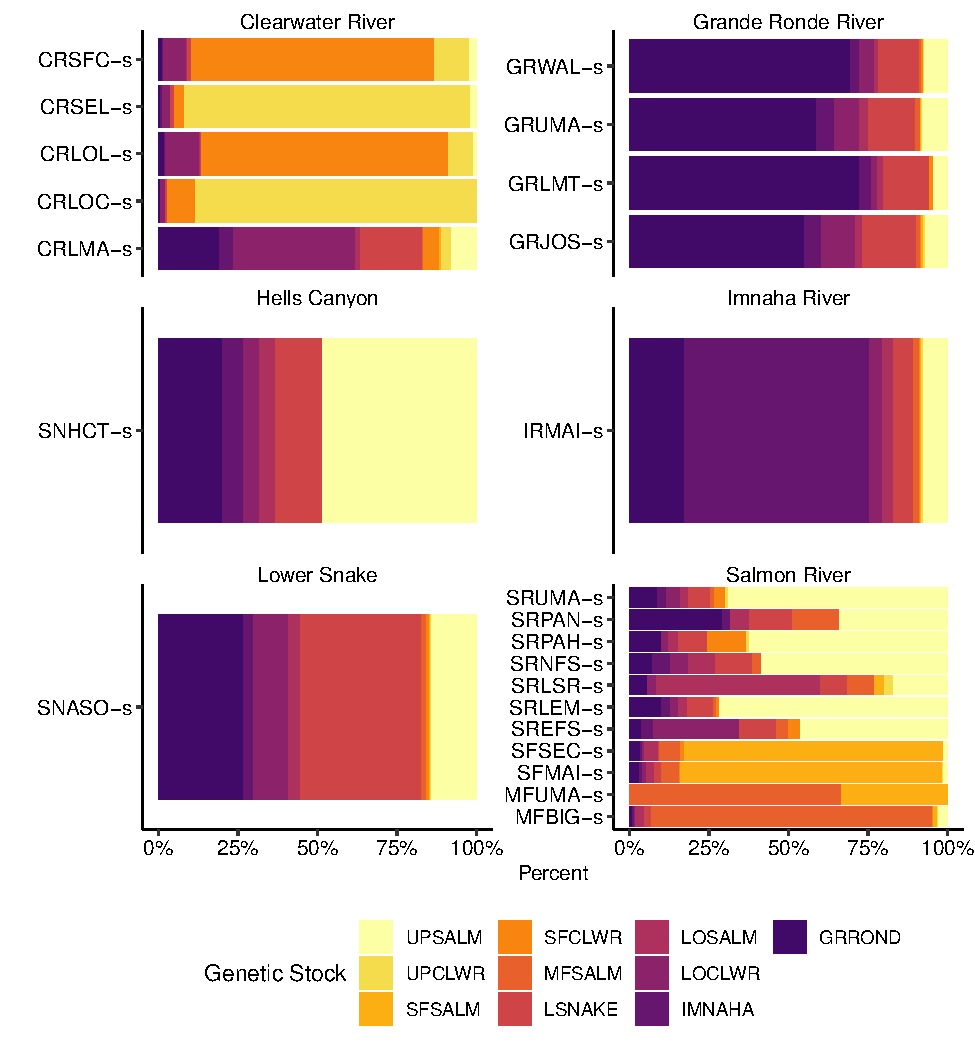
\includegraphics{Kelt_Summary_files/figure-latex/sum-gsi-1.pdf}
\caption{\label{fig:sum-gsi}Genetic stock of PIT-tagged natural-origin steelhead released at Lower Granite Dam during spawn years 2010-2020 and their final spawn location (y-axis) grouped by major population group and population.}
\end{figure}

\begin{figure}
\centering
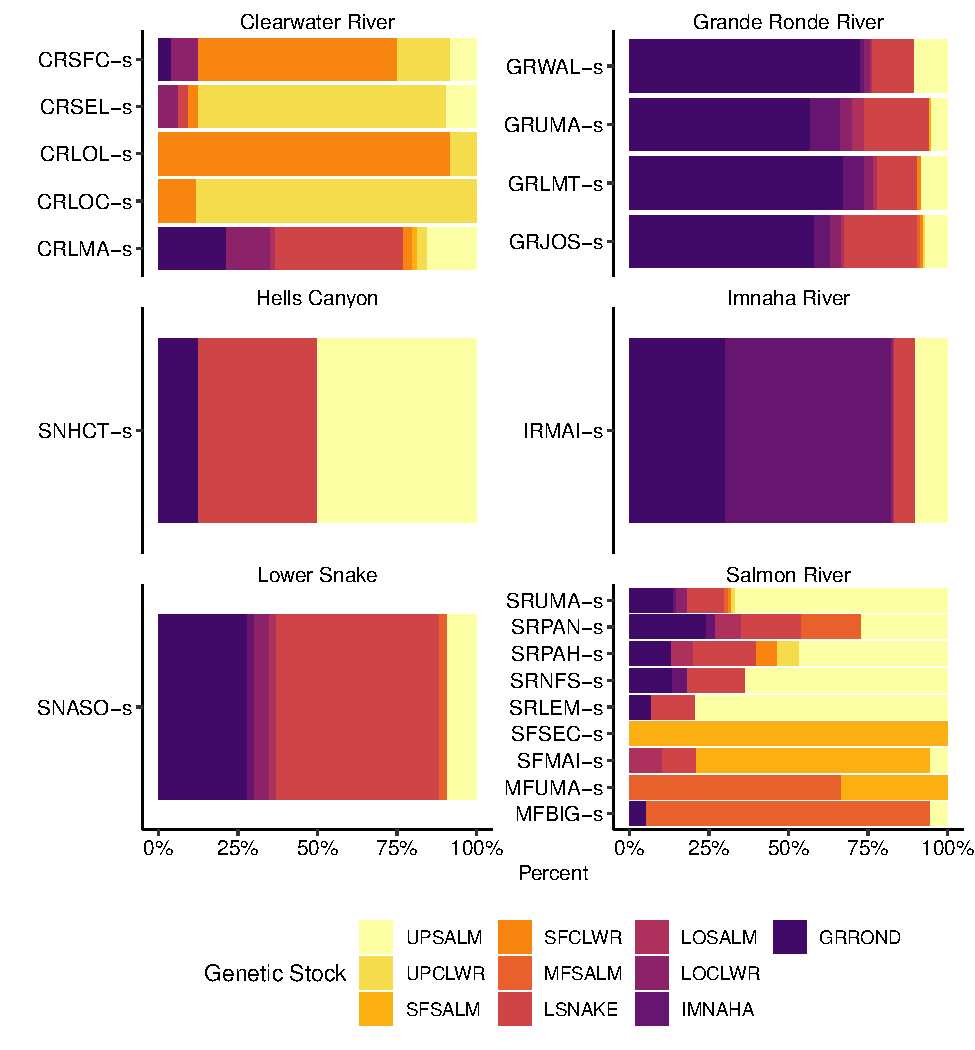
\includegraphics{Kelt_Summary_files/figure-latex/sum-gsi-sy20-1.pdf}
\caption{\label{fig:sum-gsi-sy20}Genetic stock of PIT-tagged natural-origin steelhead released at Lower Granite Dam during spawn year 2020 and their final spawn location (y-axis) grouped by major population group and population.}
\end{figure}

\begin{figure}
\centering
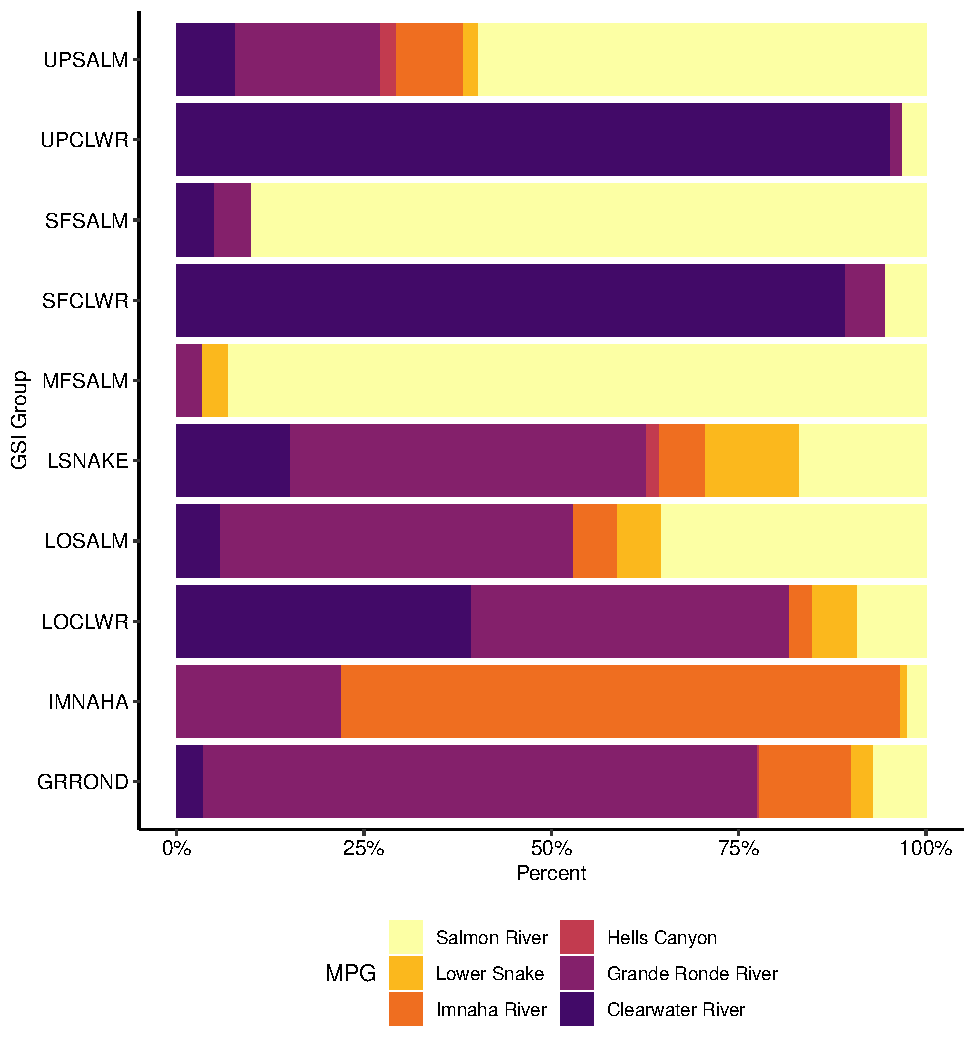
\includegraphics{Kelt_Summary_files/figure-latex/sum-gsi-mpg-1.pdf}
\caption{\label{fig:sum-gsi-mpg}Genetic stock of PIT-tagged natural-origin steelhead released at Lower Granite Dam during spawn year 2020 and their final spawn location organized by major population group and shown by color.}
\end{figure}

\begin{figure}
\centering
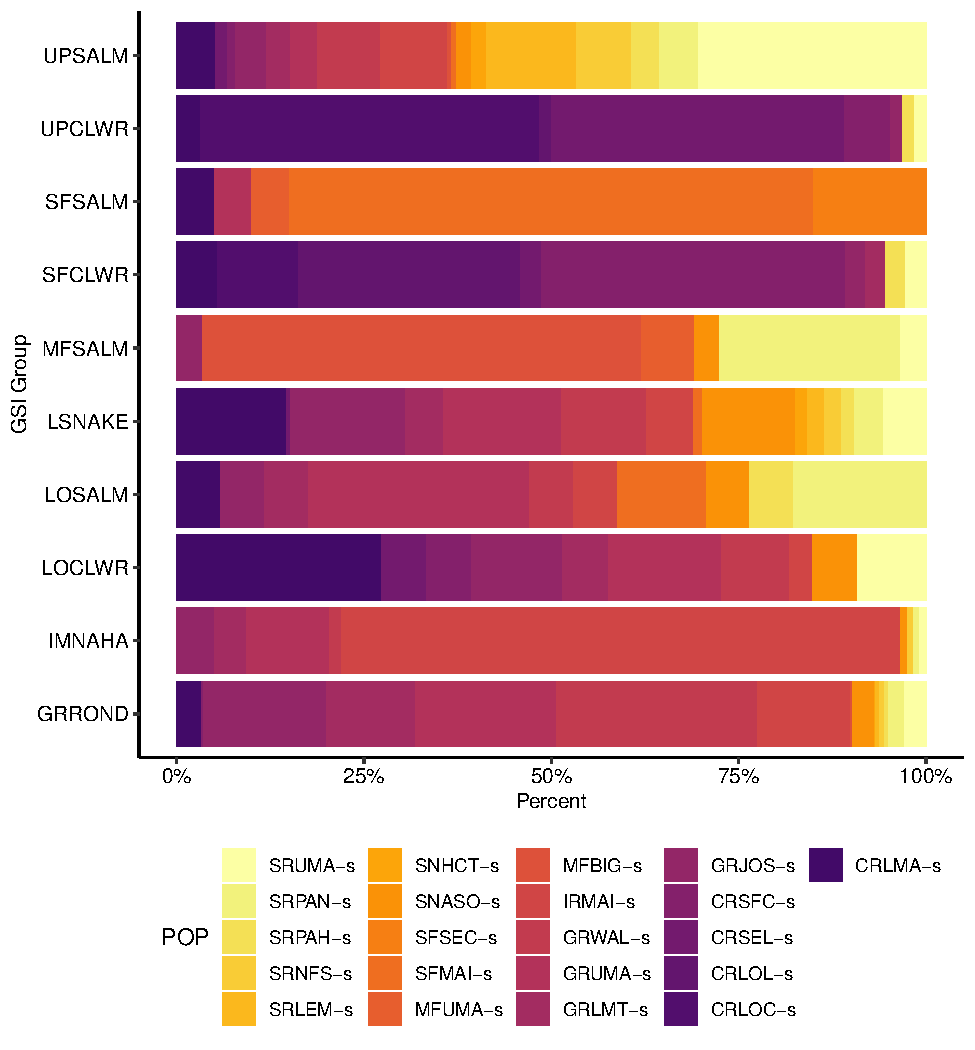
\includegraphics{Kelt_Summary_files/figure-latex/sum-gsi-pop-percent-1.pdf}
\caption{\label{fig:sum-gsi-pop-percent}Genetic stock of PIT-tagged natural-origin steelhead released at Lower Granite Dam during spawn year 2020 and their final spawn location organized by population and shown by color.}
\end{figure}

\begin{figure}
\centering
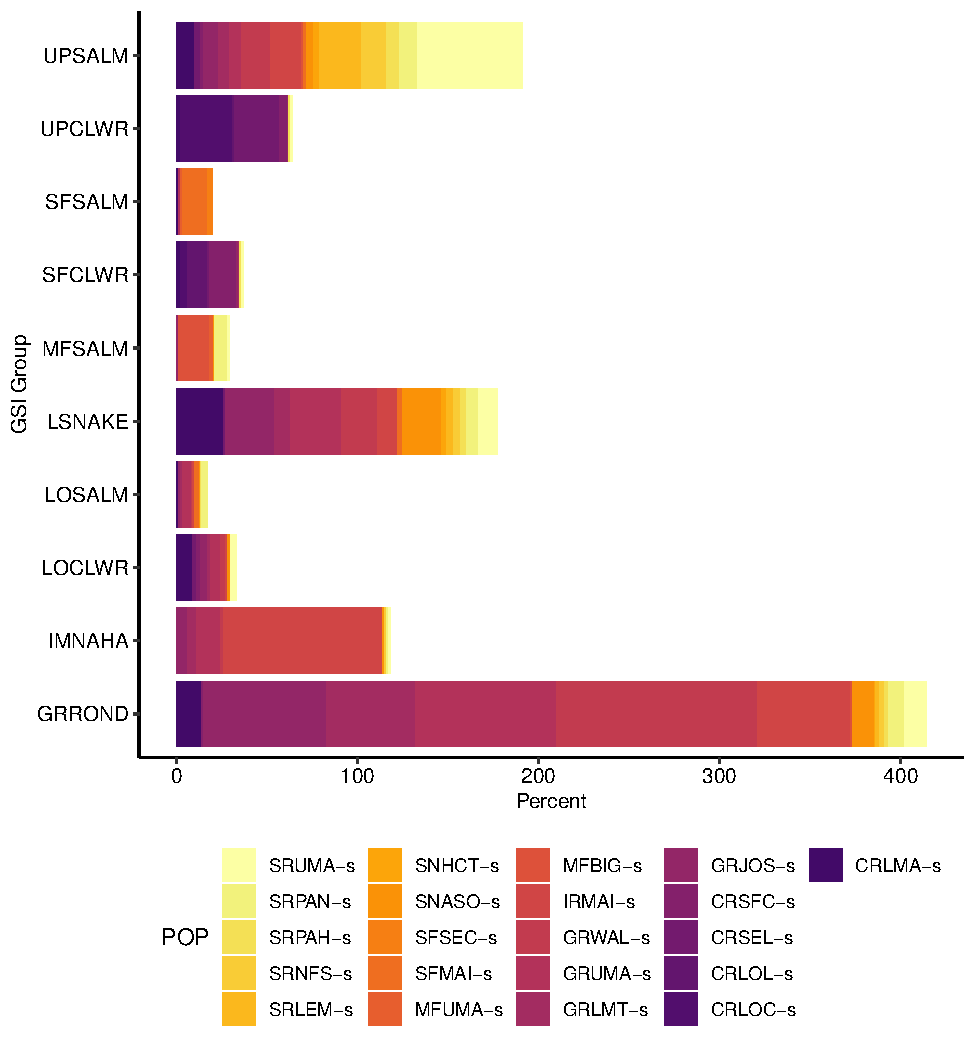
\includegraphics{Kelt_Summary_files/figure-latex/sum-gsi-pop-count-1.pdf}
\caption{\label{fig:sum-gsi-pop-count}Genetic stock of PIT-tagged natural-origin steelhead released at Lower Granite Dam during spawn year 2020 and their final spawn location organized by population and shown by color.}
\end{figure}

\begin{figure}
\centering
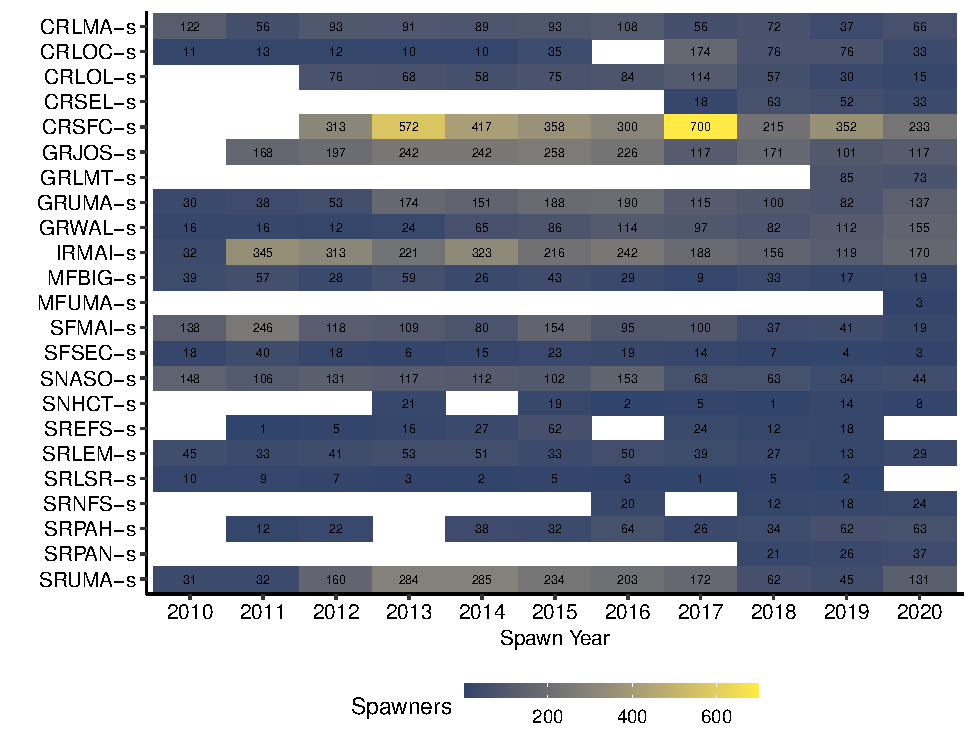
\includegraphics{Kelt_Summary_files/figure-latex/plot-pop-spawners-1.pdf}
\caption{\label{fig:plot-pop-spawners}Total PIT-tag detections of natural-origin steelhead spawning in Snake River populations upstream of Lower Granite Dam during spawn years 2010-2020.}
\end{figure}

\begin{figure}
\centering
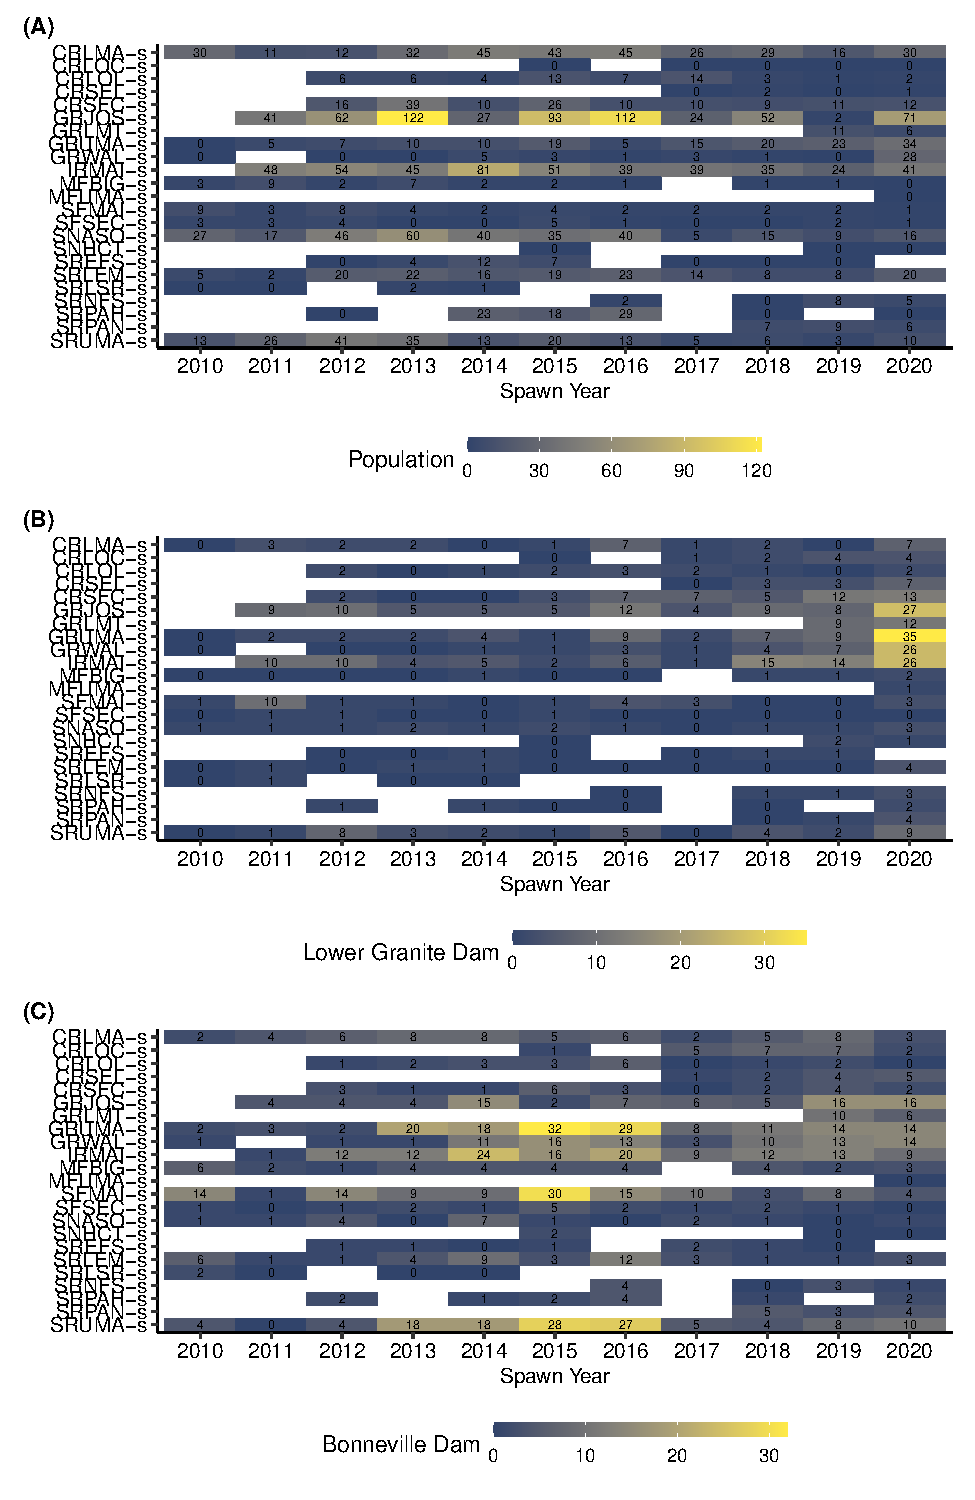
\includegraphics{Kelt_Summary_files/figure-latex/plot-observed-1.pdf}
\caption{\label{fig:plot-observed}Total PIT-tag detections of post-spawned natural-origin steelhead kelt emigrating from Sanke River populations upstream of Lower Granite Dam from spawn years 2010-2020. Panel A shows the number of kelt detected leaving population spawning areas, panel B shows the number of kelt detected at Lower Granite Dam, and panel C shows detections at Bonneville Dam.}
\end{figure}

\begin{figure}
\centering
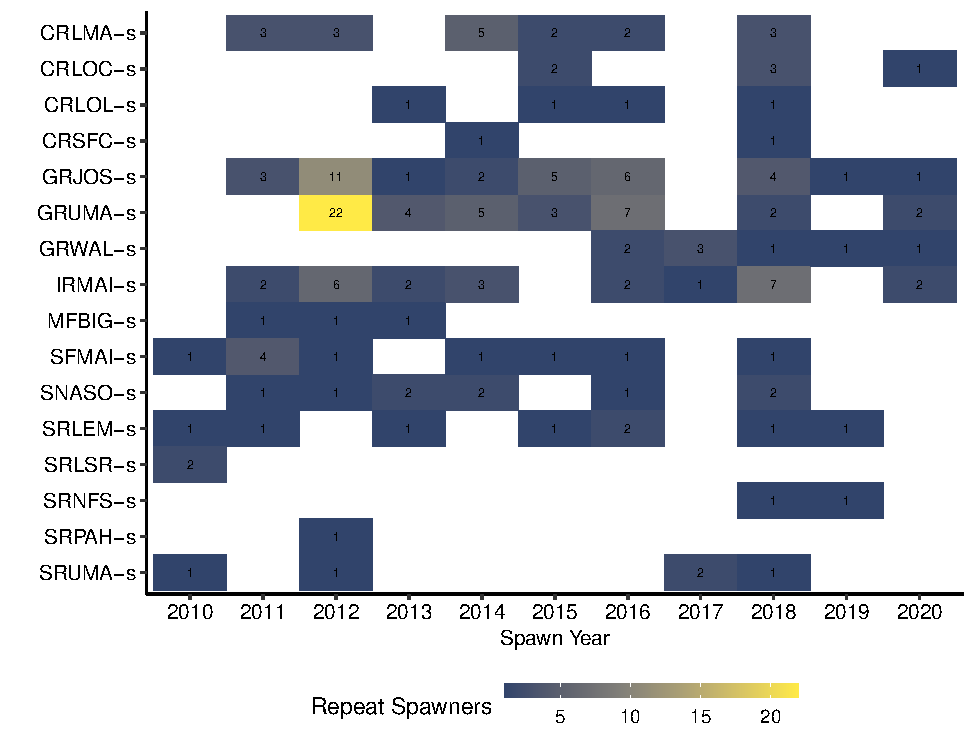
\includegraphics{Kelt_Summary_files/figure-latex/plot-pop-rs-1.pdf}
\caption{\label{fig:plot-pop-rs}Total detections of natural-origin steelhead repeat spawners originating from PIT-tagged fish released from Lower Granite Dam which spawned upstream of the dam during spawn years 2010-2020. The detection counts are grouped by population spawning area assigned during the first spawning event.}
\end{figure}

\begin{figure}
\centering
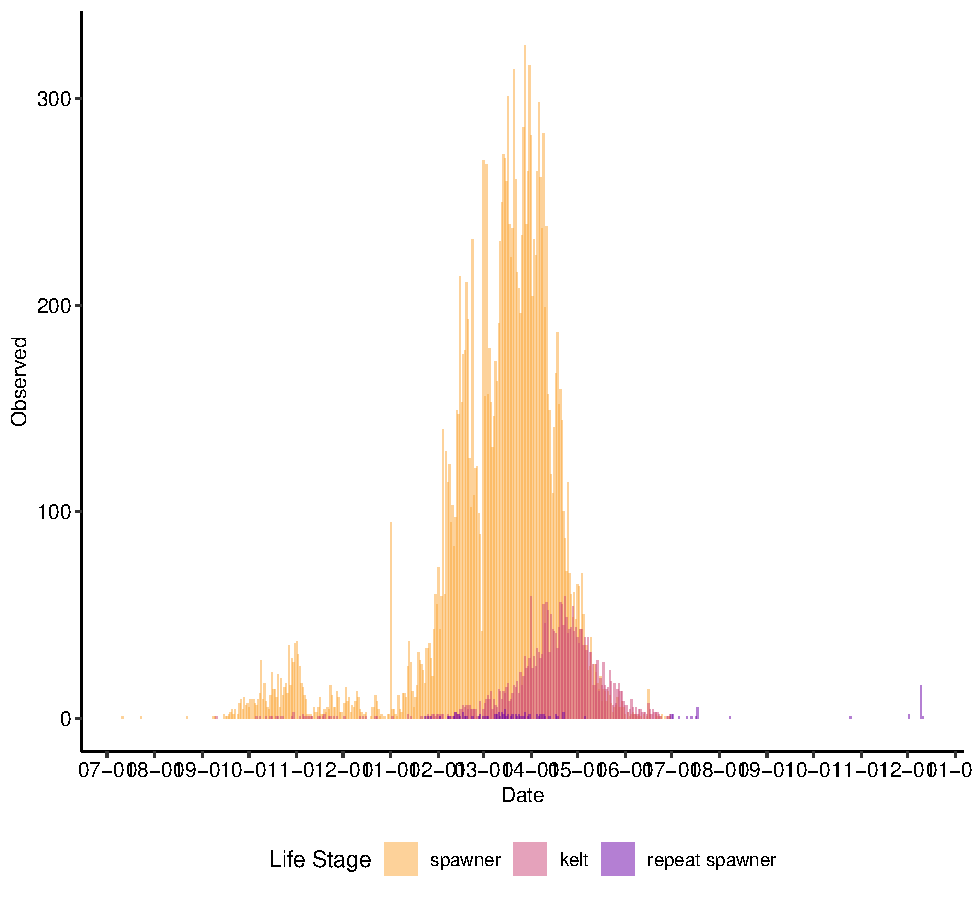
\includegraphics{Kelt_Summary_files/figure-latex/kelt-arrival-pop-1.pdf}
\caption{\label{fig:kelt-arrival-pop}Arrival distribution of PIT-tagged natural-origin steelhead to spawning locations for the three adult life-stages; spawner, post-spawned kelt, and repeat spawner. Tagged steelhead were released from the Lower Granite Dam adult trap during spawn years 2010-2020.}
\end{figure}

\begin{figure}
\centering
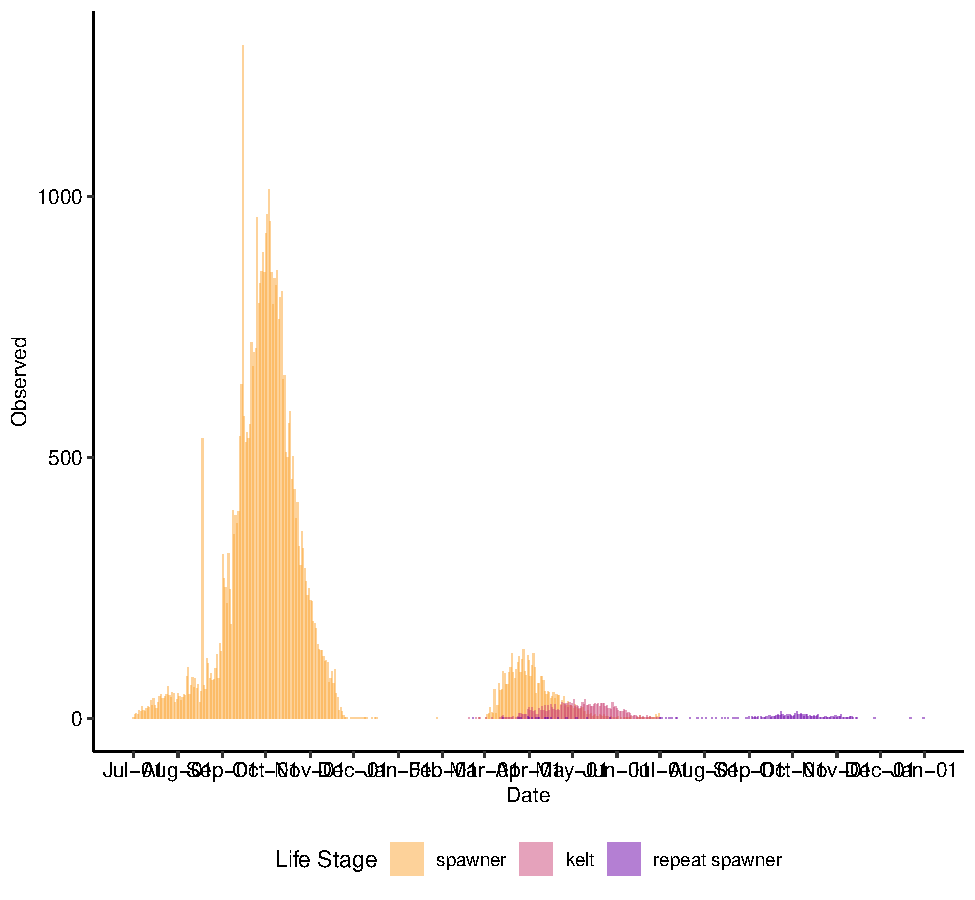
\includegraphics{Kelt_Summary_files/figure-latex/kelt-arrival-grs-1.pdf}
\caption{\label{fig:kelt-arrival-grs}Arrival distribution of PIT-tagged natural-origin steelhead to Lower Granite Dam for the three adult life-stages; spawner, post-spawned kelt, and repeat spawner. Tagged steelhead were released from the Lower Granite Dam adult trap during spawn years 2010-2020.}
\end{figure}

\begin{figure}
\centering
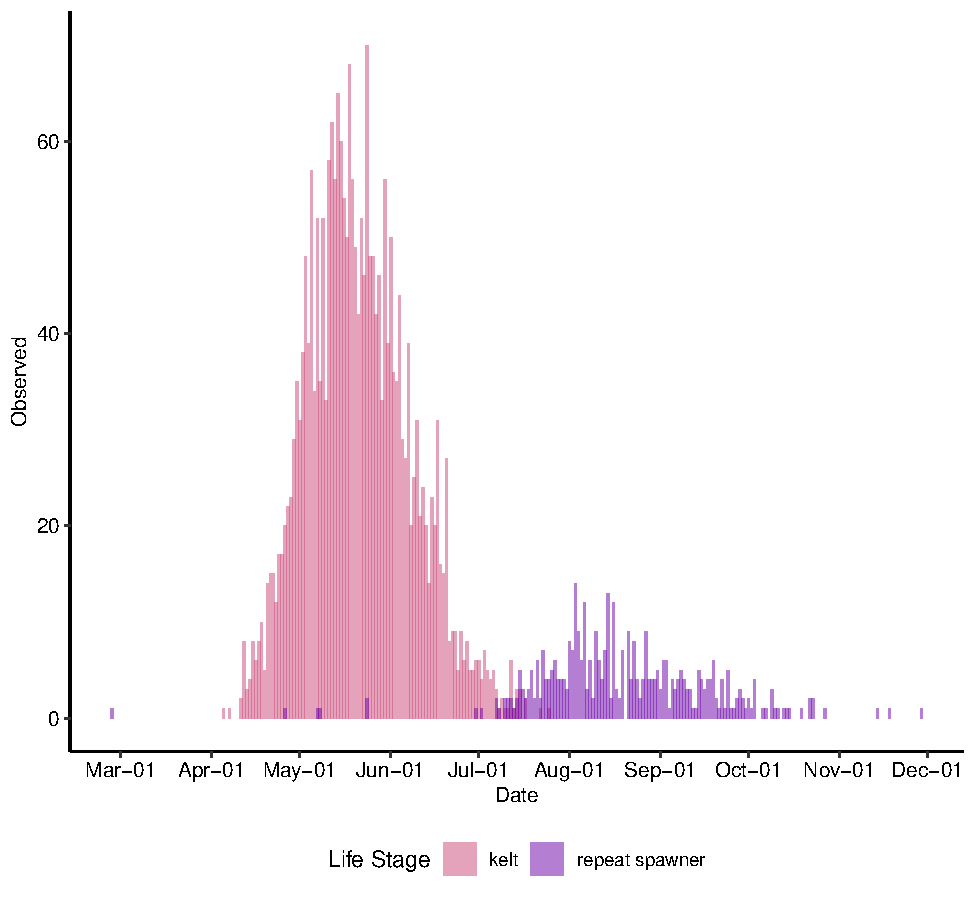
\includegraphics{Kelt_Summary_files/figure-latex/kelt-arrival-bon-1.pdf}
\caption{\label{fig:kelt-arrival-bon}Arrival distribution of PIT-tagged natural-origin steelhead for two adult life stages observed at Bonneville Dam; post-spawned kelt, and repeat spawner. Tagged steelhead were released from the Lower Granite Dam adult trap during spawn years 2010-2020.}
\end{figure}

\hypertarget{data-analysis}{%
\subsection{Data Analysis}\label{data-analysis}}

\hypertarget{discussion}{%
\section{Discussion}\label{discussion}}

\begin{itemize}
\tightlist
\item
  GSI assignment proportions are similar across spawners, kelt (all locations) and repeat spawners
\item
  Spillway weir in 2020 lead to more kelt detections at Lower Granite
\item
  Defining kelt or enumerating kelting rates at Lower Granite (i.e., in the hydrosystem) deflates the true number of fish migrating downstream as kelt and attempting to be a repeat spawner.
\item
  Lolo and SFCLW have similar kelting rates, and spawners in both locations genetically assign to SFCLWR.
\item
  Older B-run type fish in the Salmon have higher kelting rates than Clearwater B-run.
\end{itemize}

\newpage

\printbibliography

\end{document}
